\chapter{Algoritmy řešící [n,k]-Mastermind}

\section{Kategorie algoritmů}
% přidat definici algoritmu, který řeší mastermind - vytvoří posloupnost kódů, která končí tajným kódem s nejlepším ohodnocením. 
Algoritmy řešící hru Mastermind lze rozdělit do dvou kategorií, \textbf{deterministické} a \textbf{nedeterministické}. Deterministický algoritmus pro dva shodné stavy volí další krok vždy jednoznačně. Nemůže se tedy stát, že by deterministický algoritmus pro dva stejné vstupy vrátil odlišné výsledky. Nedeterministické algoritmy naproti tomu může mít v každém stavu na výběr z více následujících kroků. Volit může například podle nějakého pravděpodobnostního rozdělení. Není tedy zaručeno, že pro stejný vstup vrátí vždy stejný výsledek.

Hlavní předností deterministických algoritmů je záruka výsledku. Na druhou stranu ale tyto typy algoritmů mohou mít velikou časovou složitost, protože jsou často založeny na procházení všech možností pokračování. To se snaží řešit nedeterministické algoritmy, které hledají rovnováhu mezi časovou složitostí a dobrými výsledky. 

V této práci budeme zkoumat pouze deterministické algoritmy. 

% šlo by zmínit výhody a nevýhody (ne)deterministických algoritmů
% Popsat algoritmy, které hrají pouze kandidáty????


\section{Deterministické algoritmy}
% mozna napsat pozdeji ... Všechny deterministické algoritmy, které budeme srovnávat ...



%Tajný kód je tedy kandidát v každém kole hry. 


Definujeme orientovaný graf hry s podmnožinami $H_{n,k}$ jako vrcholy a hranami na kartézském součinu vrcholů. Nejprve popíšeme vztah mezi vrcholy, který nám bude sloužit k definování hran.
% může platit, že $(K,K_{u,r_1}) = (K,K_{v,r_2})$ pro nějaké u,v,r_1,r_2
% potomek může být i on sám. Chce to ale dobře definovat, abychom se necyklili. 
\begin{definice}[Potomek]\label{potomek}
  % Uvažujme [n,k]-Mastermind s nějakým tajným kódem $v\in H_{n,k}$. 
  Nechť $S$ je množina všech ohodnocení v $H_{n,k}$. Nechť $L$ a $K$ jsou podmnožiny $H_{n,k}$ a $ u \in H_{n,k}$ je kód. Pro $r \in S$ označíme $K_{u,r} = \{w \in K \mid s(u,w) = r\}$. 

  \begin{itemize}
      \item Řekneme, že $L$ je potomek $K$, pokud $L = K_{u,r}$ pro nějaké $u\in H_{n,k}$ a $r \in S$. 
      \item Řekneme, že $L$ je potomek $K$, vzhledem ke kódu $u$, pokud $L = K_{u,r}$ pro nějaké $r \in S$.
      \item Řekneme, že $L$ je potomek $K$, vzhledem ke kódu $u$ a ohodnocení $r$, pokud $L = K_{u,r}$.
  \end{itemize}
\end{definice}

\begin{definice}[Množina vrcholů a hran]
   Uvažujeme množinu vrcholů $\mathcal{P}(H_{n,k})$ a množinu hran $\mathcal{E}$ mezi vrcholy a jejich potomky
  \[\mathcal{E} = \{(K, L) \in \mathcal{P}(H_{n,k}) \times \mathcal{P}(H_{n,k}) \mid K \neq L, L = K_{u,r}, u \in H_{n,k}, r\in S\}\]
  Hranu $(K, K_{u,r})$ budeme značit jako hranu $(u,r)$ z vrcholu $K$.
\end{definice}


% možná to není potřeba
%\begin{lemma}[Jednoznačnost hrany]
 %   Nechť $(V, E)$ je graf a $K \in V$ je vrchol. Potom z $K$ vede právě jedna hrana 
%\end{lemma}

\begin{definice}[Cesta v grafu]\label{cesta}
    Nechť $(V, E)$ je graf [n,k]-Mastermindu a $K \in V$ je vrchol. Definujeme cestu z vrcholu $K$ jako posloupnost hran 
    \[\left((u_1, r_1), (u_2,r_2), \dots, (u_j,r_j)\right), u_i \in H_{n,k}, r_i \in \N _0 \times \N _0\]
    s první hranou začínající ve vrcholu $K$ a kde haždá hrana začíná ve stejném vrcholu, ve kterém předcházející hrana končí. Konec cesty je vrchol $L$, ve kterém končí její poslední hrana. 
\end{definice}

\begin{definice}[Graf \text{[n,k]-Mastermindu}]\label{grafmastermindu}
  Graf [n,k]-Mastermindu definujeme jako dvojici $(V, E)$, kde $V \subset  \mathcal{P}(H_{n,k})$ jsou vrcholy, do kterých vede nějaká cesta z vrcholu $H_{n,k}$ a $E = \mathcal{E} \hspace{1px} \cap V \times V$ jsou hrany na této množině. 
\end{definice}

\begin{definice}[Kandidát]
    Uvažujme [n,k]-Mastermind s nějakým tajným kódem $v\in H_{n,k}$. Nechť 
    \[P = \left((u_1, r_1), (u_2,r_2), \dots, (u_j,r_j)\right), u_i \in H_{n,k}, r_i \in \N _0 \times \N _0\]
    jsou tahy s ohodnocením. Řekneme, že $u \in H_{n,k}$ je kandidát, pokud $u \in K$, kde $K$ je konec cesty $P$ z vrcholu $H_{n,k}$.
\end{definice}


% tato definice možná ani není potřeba, protože s ní dále nepracuji
\begin{definice}[Rozdělení]
    Pro $K \subset H_{n,k}$ definujeme rozdělení vzhledem ke kódu $u$ jako množinu potomků $K$, vzhledem ke kódu $u$. $R_{K,u} = \{K_{u,r} \mid r \in S\}$. 
\end{definice}

\begin{definice}[Jednokroková funkce]
    Nechť $G = (V,E)$ je graf [n,k]-Mastermindu a $K \in V$ je vrchol. Potom jednokroková funkce $f_K(u) \colon H_{n,k} \to \mathbb{R}$ je taková, která kódu $u$ přiřadí hodnotu, která lze vyjádřit pomocí potomků $K$ vzhledem ke kódu $u$.
\end{definice}

\begin{prikl}\label{prjednokrokfce}
    Funkce $f_K$ níže je jednokroková funkce.
    \begin{align*}
        f_K \colon H_{n,k} &\to \mathbb{R} \\
        u &\mapsto \sum_{r\in S}\frac{|K_{u,r}|}{|K|}|K_{u,r}| 
    \end{align*}
    Navíc $\forall u \in H_{n,k} \colon \hspace{3px} K = \bigcup_{r\in S} K_{u,r}$.
\end{prikl}

\begin{definice}[Funkcionál]
    Nechť $A$ je konečná množina a $\mathcal{F} = \{f\colon A \to \mathbb{R}\}$ je prostor funkcí. Potom funkcionálem nazveme zobrazení $F \colon \mathcal{F} \to \mathbb{R}$. 
\end{definice}

\begin{prikl}\label{prfunkcional}
    Nechť $A$ je konečná množina a $\mathcal{F} = \{f\colon A \to \mathbb{R}\}$ je prostor funkcí. Potom funkcionál definovaný na $\mathcal{F}$ může být například
    \begin{align*}
        F \colon \mathcal{F} &\to \mathbb{R} \\
        f &\mapsto \max\{f(a) \mid a\in A\}
    \end{align*}
    Funkcionál je dobře definovaný, protože maximum na konečné množině reálných čísel má vždy jednoznačnou hodnotu.
\end{prikl}

% \subsection{Varianty algoritmů}


\subsubsection{Jednokrokové algoritmy}
Jednokrokové algoritmy definujeme následovně. Nechť $G = (V,E)$ je graf [n,k]-Mastermindu.
Nechť $\mathcal{F} = \{f_K \mid K \in V \} $ je prostor jednokrokových funkcí, kde $f_K \colon H_{n,k} \to \mathbb{R}$ jsou jednokrokové funkce. Nechť $F$ je funkcionál na $\mathcal{F}$. Potom jednokrokový algoritmus s prostorem funkcí $\mathcal{F}$ a funkcionálem $F$ je definovaný v algoritmu \ref{jednokrokalgorithm}. 




%Nechť \[P = \left((u_1, r_1), (u_2,r_2), \dots, (u_j,r_j)\right), u_i \in H_{n,k}, r_i \in \N _0 \times \N _0\] jsou tahy s ohodnocením a $K$ je konec cesty $P$ z vrcholu $H_{n,k}$. 

%Potom jednokrokové strategie volí další kód ten, který minimalizuje respektive maximalizuje funkci $f_K$. Pokud je těchto kódů více, zvolí kód, který je zároveň kandidát cesty $P$. Pokud výběr stále není jednoznačný, algoritmus zvolí lexikograficky nejnižší kód. 

\begin{algorithm}[h!]
\begin{algorithmic}[1]  % [1] způsobí, že číslujeme kroky algoritmu
\Function{one-step-algorithm}{$n,k,s_v,\mathcal{F},F$}
    \State $K \gets H_{n,k}$ 
    \State $j \gets 0$
    \State $r_0 \gets (0,0)$
    \While {$r_j \neq (n,0)$} \hfill \mbox{(dokud hra není dohrána)}
        \State $j \gets j + 1$ 
	\State $U \gets \{u \in H_{n,k} \mid f_K(u) = F(f_K)\}$
        \If{$U \cap K \neq \emptyset$}
            \State $u_j \gets$ lexikograficky nejmenší $u \in U \cap K$
	\Else
		\State $u_j \gets$ lexikograficky nejmenší $u \in U$
	\EndIf
        \State $r_j \gets s_v(u_j)$ \hfill \mbox{(ohodnocení pokusu)}
        \State $K \gets K_{u_j,r_j}$
    \EndWhile
    \State Vrátíme $u_j, j$ \hfill \mbox{($u_j$ je tajný kód, $j$ je počet pokusů)}
\EndFunction
\end{algorithmic}
\caption{Jednokrokový algoritmus řešící [n,k]-Mastermind}
\label{jednokrokalgorithm}
\end{algorithm}

Písmenem $K$ značíme množinu kandidátů pro aktuální průběh hry (cestu). ve druhém řádku položíme $K = H_{n,k}$, protože tajným kódem mohou být všechny kódy. Aktuální číslo pokusu značí $j$, $u_j$ je kód, který algoritmus zvolí jako $j$-tý pokus a $r_j$ je ohodnocení $u_j$ vzhledem k tajnému kódu $v$. Množina $U$ značí kódy, ve kterých funkce $f_K$ nabývá určitou optimální hodnotu danou funkcionálem $F$. Z této množiny algoritmus vybírá další pokus $u_j$. Ve chvíly, kdy existuje kandidát v množině $U$ ($U\cap K \neq \emptyset$), algoritmus zvolí ten lexikograficky nejmenší. Jinak algoritmus volí lexikograficky nejmenší kód z $U$. 

Aby byl funkcionál $F$ použitelný v algoritmu, musí platit následující podmínka. 
\[\forall K \in V \hspace{5px} \exists u \in H_{n,k} \colon F(f_K) = f_K(u)\]
Pokud by tato podmínka nebyla splněna, mohlo by se stát, že množina $U$ bude prázdná a algoritmus nedokáže zvolit další pokus.

% šlo by napsat pro dvojice funkce f, funkcionál F
%\begin{veta}[Správnost algoritmu \ref{jednokrokalgorithm}]
 %   Algoritmus \ref{jednokrokalgorithm}
%\end{veta}




\begin{figure}[h!]
    \centering
    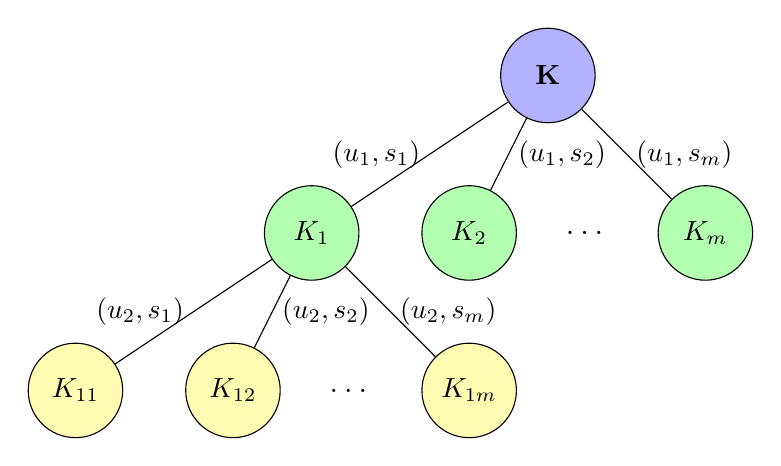
\begin{tikzpicture}
    \node[draw, circle, fill=blue!30, minimum size=12mm] (1) at (0,0) {\textbf{K}};
    
    \node[draw, circle, fill=green!30, minimum size=12mm] (2) at (-3,-2) {$K_1$};
    \draw (1) -- (2) node[pos=0.5, left] {$(u_1,s_1)$};
    \node[draw, circle, fill=green!30, minimum size=12mm] (3) at (-1,-2) {$K_2$};
    \draw (1) -- (3) node[pos=0.5, right] {$(u_1,s_2)$};
    \node[draw, circle, fill=green!30, minimum size=12mm] (5) at (2,-2) {$K_m$};
    \draw (1) -- (5) node[pos=0.5, right] {$(u_1,s_m)$};
    \node (4) at (0.5,-2) {\large \dots};


    \node[draw, circle, fill=yellow!30, minimum size=12mm] (6) at (-6,-4) {$K_{11}$};
    \draw (2) -- (6) node[pos=0.5, left] {$(u_2,s_1)$};
    \node[draw, circle, fill=yellow!30, minimum size=12mm] (7) at (-4,-4) {$K_{12}$};
    \draw (2) -- (7) node[pos=0.5, right] {$(u_2,s_2)$};
    \node (8) at (-2.5,-4) {\large \dots};
    \node[draw, circle, fill=yellow!30, minimum size=12mm] (9) at (-1,-4) {$K_{1m}$};
    \draw (2) -- (9) node[pos=0.5, right] {$(u_2,s_m)$};
    
    \end{tikzpicture}
    \caption{Strom o dvou tazích}
    \label{figcandidatetree}
    \end{figure}



V této kapitole porovnáme tři jednokrokové algoritmy, které se liší pouze podle zvoleného prostoru jednokrokových funkcí a funkcionálu. 
% Nějak popsat to, jak odhadujeme výsledný počet tahů podle tabulky rozdělení - max, entropie, počet částí, očekávaná velikost části v tabulce rozdělení - Irwing, nezmínil jsem.

\subsection{min-max}
\begin{definice}[Maximum rozdělení]
    Nechť $H_{n,k}$ je prostor kódů. Pro $K \subset H_{n,k}$ definujeme funkci maximum rozdělení jako
    \begin{align*}
        m_K \colon H_{n,k} &\to \mathbb{R} \\
        u &\mapsto \max_{r\in S}\{|K_{u,r}|\}.
    \end{align*}
    Prostor všech funkcí $m_K$ označíme $\mathcal{M}$. 
\end{definice}

\begin{definice}[Funkcionál minimum]
    Nechť $H_{n,k}$ je prostor kódů a $\mathcal{F} = \{f_K\colon H_{n,k} \to \mathbb{R} \mid K \subset H_{n,k}\}$ je prostor funkcí. Potom definujeme funkcionál minimum definovaný na $\mathcal{F}$ jako
    \begin{align*}
        L \colon \mathcal{F} &\to \mathbb{R} \\
        f &\mapsto \min_{u\in H_{n,k}}\{f(u)\}
    \end{align*}
\end{definice}

Prvním algoritmem je metoda, kterou navrhl D. Knuth \cite{donald_e__knuth_1977}. Odpovídá algoritmu \ref{jednokrokalgorithm} se vstupním prostorem funkcí $\mathcal{M}$ a funkcionálem $L$. Jeho algoritmus tedy vybírá pro další pokus ten kód, který minimalizuje maximální počet kódů v potomcích vzhledem k nějakému kódu. Tedy v každém kroku algoritmu \ref{jednokrokalgorithm} pro množinu kandidátů $K$ bude vybírat kód z množiny 
\[U = \{u \in H_{n,k} \mid m_K(u) = L(m_K)\}\]
tedy
\[U = \{u \in H_{n,k} \mid \max_{r\in S}\{|K_{u,r}| \} = \min_{w \in H_{n,k}}\{\max_{r\in S}\{|K_{w,r}|\} \} \}\]



Chod Knuthova algoritmu nastíníme na [2,2]-Mastermindu. 
\subsubsection{[2,2]-Mastermind}
Prostor kódů [2,2]-Mastermindu je množina $H_{2,2} = \{11,12,21,22\}$. Množina všech ohodnocení je podle tvrzení \ref{tvrzohodnoceni2} rovna $S = \{(0,0), (0,2), (1,0), (2,0)\}$. Na obrázku \ref{fig22prvnitah11} a \ref{fig22prvnitah12} jsou zobrazeny potomci $H_{2,2}$ vzhledem ke kódu $11$ a $12$. Případy s kódy $22$ a $21$ jsou obdobné zmíněným kódům díky rovnoměrnému rozdělení kódů. Protože kódy $22$ a $21$ jsou lexikograficky vyšší, nemusíme je rozebírat. 
\begin{figure}[h!]
    \centering
    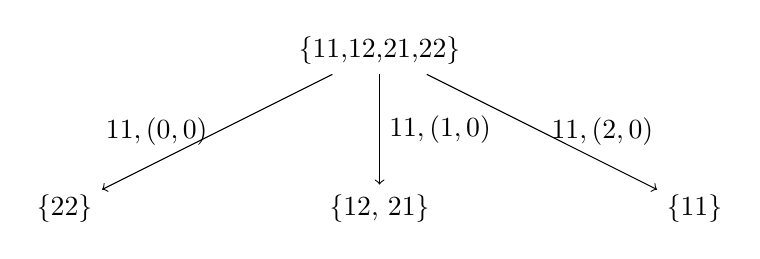
\begin{tikzpicture}
    \node (1) at (0,0) {\{11,12,21,22\}};
    
    \node (2) at (-4,-2) {\{22\}};
    \draw[->] (1) -- (2) node[pos=0.5, left] {$11,(0,0)$};
    \node (3) at (0,-2) {\{12, 21\}};
    \draw[->] (1) -- (3) node[pos=0.5, right] {$11,(1,0)$};
    \node (5) at (4,-2) {\{11\}};
    \draw[->] (1) -- (5) node[pos=0.5, right] {$11,(2,0)$};

    \end{tikzpicture}
    \caption{První tah, obdobný s grafem pro 22}
    \label{fig22prvnitah11}
    \end{figure}
\begin{figure}[h!]
    \centering
    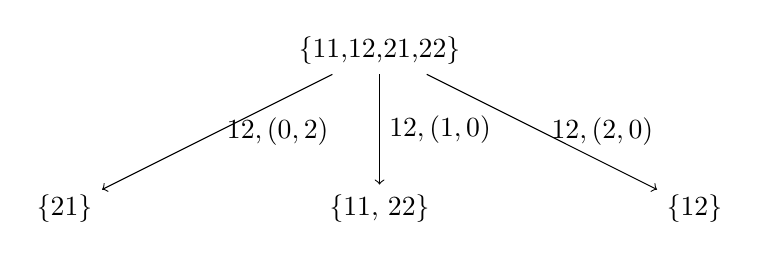
\begin{tikzpicture}
    \node (1) at (0,0) {\{11,12,21,22\}};
    
    \node (4) at (-4,-2) {\{21\}};
    \draw[->] (1) -- (4) node[pos=0.5, right] {$12,(0,2)$};
    \node (5) at (0,-2) {\{11, 22\}};
    \draw[->] (1) -- (5) node[pos=0.5, right] {$12,(1,0)$};
    \node (6) at (4,-2) {\{12\}};
    \draw[->] (1) -- (6) node[pos=0.5, right] {$12,(2,0)$};

    \end{tikzpicture}
    \caption{První tah, obdobný s grafem pro 21}
    \label{fig22prvnitah12}
\end{figure}

Hodnoty $m_{H_{2,2}}$ jsou tedy následující. 
\[m_{H_{2,2}} (11) = m_{H_{2,2}} (12) = m_{H_{2,2}} (21) = m_{H_{2,2}} (22) = 2\]
Knuthův algoritmus volí jako první pokus kód $11$. 
\begin{figure}[h!]
    \centering
    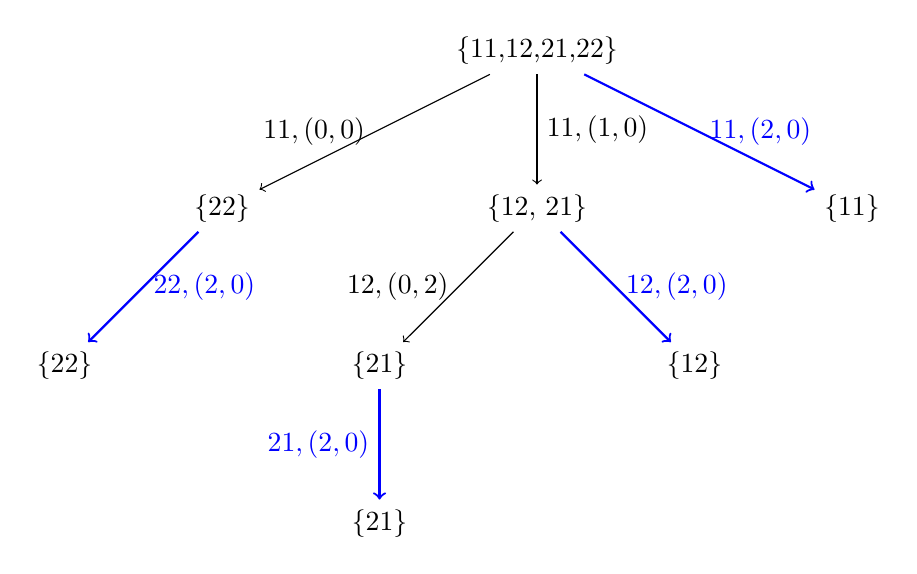
\begin{tikzpicture}
    \node (1) at (0,0) {\{11,12,21,22\}};
    \node (2) at (-4,-2) {\{22\}};
    \draw[->] (1) -- (2) node[pos=0.5, left] {$11,(0,0)$};
    \node (3) at (0,-2) {\{12, 21\}};
    \draw[->] (1) -- (3) node[pos=0.5, right] {$11,(1,0)$};
    \node (4) at (4,-2) {\{11\}};
    \draw[->, thick, blue] (1) -- (4) node[pos=0.5, right] {$11,(2,0)$};
    \node (5) at (-2,-4) {\{21\}};
    \draw[->] (3) -- (5) node[pos=0.5, left] {$12,(0,2)$};
    \node (6) at (2,-4) {\{12\}};
    \draw[->, thick, blue] (3) -- (6) node[pos=0.5, right] {$12,(2,0)$};
    \node (7) at (-6,-4) {\{22\}};
    \draw[->, thick, blue] (2) -- (7) node[pos=0.5, right] {$22,(2,0)$};
    \node (8) at (-2,-6) {\{21\}};
    \draw[->, thick, blue] (5) -- (8) node[pos=0.5, left] {$21,(2,0)$};
    \end{tikzpicture}
    \caption{První a druhý tah}
\label{fig22dvatahy}
\end{figure}

Na obrázku \ref{fig22dvatahy} jsou doplněny potomci všech vrcholů až do dosažení ohodnocení $(2,0)$, kdy hra končí. Platí, že $m_K(u) \geq 1$ pro $K \neq \emptyset$. Proto, když lexikograficky nejnižší kandidát $u$ dosahuje hodnoty $m_K(u) = 1$, algoritmus min-max ho vždy vybere. Ukazuje se, že to je případ pro všechny zbývající vrcholy, $\{22\}, \{12, 21\}, \{21\}$.
    
\begin{figure}[h!]
    \centering
    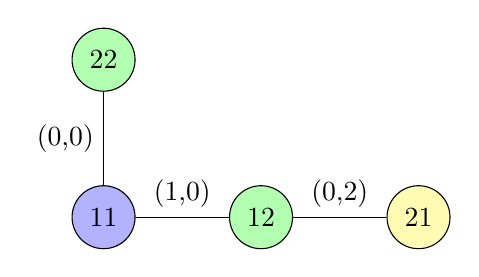
\begin{tikzpicture}
    \node[draw, circle, fill=blue!30, minimum size=8mm] (1) at (0,0) {11};
    \node[draw, circle, fill=green!30, minimum size=8mm] (2) at (0,2) {22};
    \draw (1) -- (2) node[pos=0.5, left] {(0,0)};
    \node[draw, circle, fill=green!30, minimum size=8mm] (3) at (2,0) {12};
    \draw (1) -- (3) node[pos=0.5, above] {(1,0)};
    \node[draw, circle, fill=yellow!30, minimum size=8mm] (4) at (4,0) {21};
    \draw (3) -- (4) node[pos=0.5, above] {(0,2)};
    
    \end{tikzpicture}
    \caption{Zahrané tahy podle ohodnocení}
    \label{fig23start12}
\end{figure}




% Přidat pseudokód algoritmu???

%vysledky Knuthova algoritmu:
% zdroj - Kooi
%expected - 4.476
% maximal - 5
% použít svůj kód a ocitovat

\subsection{entropie}
\begin{definice}[Entropie rozdělení]
    Nechť $H_{n,k}$ je prostor kódů. Pro $K \subset H_{n,k}$ definujeme funkci entropie rozdělení jako
    \begin{align*}
        h_K \colon H_{n,k} &\to \mathbb{R} \\
        u &\mapsto \sum_{r\in S} \frac{|K_{u,r}|}{|K|}\log_2\left( \frac{|K|}{|K_{u,r}|} \right)
    \end{align*}
    Prostor všech funkcí $h_K$ označíme $\mathcal{H}$. 
\end{definice}

\begin{definice}[Funkcionál maximum]
    Nechť $H_{n,k}$ je prostor kódů a $\mathcal{F} = \{f_K\colon H_{n,k} \to \mathbb{R} \mid K \subset H_{n,k}\}$ je prostor funkcí. Potom definujeme funkcionál minimum definovaný na $\mathcal{F}$ jako
    \begin{align*}
        M \colon \mathcal{F} &\to \mathbb{R} \\
        f &\mapsto \max_{u\in H_{n,k}}\{f(u)\}
    \end{align*}
\end{definice}

Neuwirth \cite{neuwirth} 
% Asi Neuwirth, chtělo by ale najít článek Irwinga.
navrhl algoritmus hrající tahy, které maximalizují entropii tabulky rozdělení. Nejprve však musíme definovat, co si vlastně pod entropií tabulky rozdělení můžeme představit a jaký má pro nás entropie význam.

\begin{definice}[Entropie]\label{defentropie}
  Nechť $A$ je konečná množina, $P \colon A \to [0,1]$ je zobrazení takové, že $\sum_{a \in A} P(a) = 1$. Nechť $s(P) = \{ a \in A \mid P(a) > 0\}$. Potom entropii zobrazení $P$ definujeme jako 
  \[H(P) = \sum_{a \in s(P)}P(a)\log_2\left(\frac{1}{P(a)}\right)\]
  Zobrazení $P$ budeme říkat rozdělení, dané hodnotě $P(a)$ pravděpodobnost a množině $[0,1]$ pravděpodobnostní prostor. 
\end{definice}

\begin{definice}[Entropie tabulky rozdělení]\label{defentropietabrozdel}
  Uvažujme [n,k]-Mastermind s tajným kódem $v$. Nechť $K$ množina kandidátů, $u \in H_{n,k}$ a $K^u = (|K^u_1|, |K^u_1|, \dots, |K^u_m|)$ je jeho tabulka rozdělení. Potom entropii tabulky rozdělení definujeme jako
  \[H(K^u) = \sum_{i=1}^n \frac{|K^u_i|}{|K|}\log_2\left( \frac{|K|}{|K^u_i|} \right)\]
\end{definice}

\begin{pozn}
    Definice \ref{defentropietabrozdel} koresponduje s definicí entropie pro množinu všech ohodnocení $A = \{s_1, s_2, \dots, s_m \}$ a zobrazení $P\colon A \to [0,1], P(s_i) = \frac{|K^u_i|}{|K|}$.
\end{pozn}

Co nám ale tato definice říká? Intuici za definicí entropie nastíníme v příkladu \ref{prbinarysearch}, který dává určitou smysl pro výraz $\log_2\left(\frac{1}{P(a)}\right)$ a příkladu \ref{prentropierozdeleni}, který ukazuje příklad entropie na konkrétním rozdělení.

Představme si, že chceme uhodnout tajné číslo z množiny $\{1,2,\dots,8\}$ pokládáním nějakých ano/ne otázek. Předpokládejme, že každé číslo může být tajným číslem se stejnou pravděpodobností $\frac{1}{8}$. Známým postupem, jak tajné číslo najít je takzvaným půlením intervalu (binární vyhledávání). Vždy se zeptáme, zda je číslo větší nebo menší než číslo v polovině. Tento postup je znázorněn v příkladu \ref{prbinarysearch}.

\begin{prikl}[Binární vyhledávání]\label{prbinarysearch}
Nechť tajné číslo je 4. Binární vyhledávání by mělo následující průběh:

Otázka: "Je číslo větší než 4?". 
Odpověď: ne

Otázka: "Je číslo větší než 2?". 
Odpověď: ano

Otázka: "Je číslo větší než 3?". 
Odpověď: ano

Výsledné číslo je 4. Počet otázek nutných k určení tajného čísla je 3.
\end{prikl}

\begin{pozn}\label{poznotazkynamnozinu}
Obdobně jako v příkladu \ref{prbinarysearch} lze pro jakoukoliv osmiprvkovou množinu $A$ s rovnoměrnou pravděpodobností vytvořit sadu otázek ano/ne a o každém prvku této množiny určit, zda odpovídá odpovědi ano nebo odpovědi ne. Následně bychom mohli pro určení jakéhokoliv prvku této množiny aplikovat obdobný postup jako v příkladu \ref{prbinarysearch}. Pro vhodnou sadu otázek existuje postup, který každou otázkou rozdělí prostor zbývajících možností na polovinu. Tím pádem pro určení jakéhokoliv prvku množiny $A$ potřebujeme $\log_2(|A|)$ otázek. 
\end{pozn}

\begin{prikl}\label{prentropierozdeleni}
Nechť $A = \{ \text{a, b, c, d}\}$ a $P$ je zadaná následovně: 
\[P(a) = \frac{1}{8}, P(b) = \frac{1}{8}, P(c) = \frac{1}{4}, P(d) = \frac{1}{2}\]
Nyní si představme pravděpodobnostní prostor jako čtverec na obrázku \ref{prprostor}, kde pravděpodobnost prvku je velikost plochy. Výraz $\frac{1}{P(a)}$ říká, kolik prvků $A$ s touto pravděpodobností by se "vešlo" do pravděpodobnostního prostoru jako na obrázku. Například dílek c by se "vešel" do pravděpodobnostního prostoru čtyřikrát.
Hodnota $\log_2\left(\frac{1}{P(c)}\right)$ lze interpretovat jako počet otázek ano/ne, který potřebujeme k jednoznačnému určení prvku c v případě, kdyby byl pravděpodobnostní prostor rozdělen rovnoměrně. Tento postup byl popsán v příkladu \ref{prbinarysearch} a v diskuzi pod ním.
Entropie tohoto rozdělení by v tomto případě byla 
\[H(P) = \frac{1}{8}\log_2 (8) + \frac{1}{8}\log_2 (8) + \frac{1}{4}\log_2 (4) + \frac{1}{2}\log_2 (2) = \frac{3}{8} + \frac{3}{8} + \frac{2}{4} + \frac{1}{2} = \frac{7}{4}\]
a můžeme ji interpretovat jako vážený průměr počtu otázek, který potřebujeme k jednoznačnému určení prvku z množiny $A$. 


\begin{figure}
\begin{tikzpicture}
    \draw[black, thick] (0,0) rectangle (4,4);
    \begin{scope}
        \node (1) at (1,0.5) {a - 1/8}
        \node (2) at (1,1.5) {b - 1/8}
        \node (3) at (1,3) {c - 1/4}
        \node (4) at (3,2) {d - 1/2}
    \end{scope}
    \draw[black, thick] (2,0) -- (2,4);
    \draw[black, thick] (0,2) -- (2,2);
    \draw[black, thick] (0,1) -- (2,1);

    
\end{tikzpicture}
\caption{Pravděpodobnostní prostor}
\label{prprostor}
\end{figure}

\end{prikl}

Nyní jsme připraveni na to, abychom vysvětlili, jakým způsobem aplikujeme výpočet entropie na strategii pro řešení [4,6]-Mastermindu.

Nechť $K$ je aktuální množina kandidátů, $u \in H_{4,6}$ je kód a $(|K_1|, |K_2|,\dots, |K_m|)$ je tabulka rozdělení pro kód $u$. Pro každé $K_i, i \in \{1, 2, \dots, m\}$ můžeme ve smyslu poznámky \ref{poznotazkynamnozinu} definovat nějakou abstraktní hodnotu počtu otázek ano/ne potřebných k určení jakéhokoliv prvku  $x \in K_i$ jako $\log_2(|K_i|)$. Potom obdobně jako v příkladu \ref{prentropierozdeleni} můžeme určit očekávaný počet otázek jako
\[G = \sum_{i =1}^n \frac{|K_i|}{|K|}\log_2|K_i| \]
Tato hodnota bude naším stavebním kamenem pro strategii za užití entropie. Protože cílem [4,6]-Mastermindu je najít tajný kód v co nejmenším počtu pokusů, chceme hodnotu $G$ minimalizovat. 

\[ u = \arg\min_{w \in H_{4,6}} \sum_{i =1}^n \frac{|K_i|}{|K|}\log_2|K_i|\]

\begin{lemma}[Aritmetika min a max]
    Nechť $K$ je konečná množina a $f \colon K \to \mathbb{R}$ je funkce. Nechť $a \in \mathbb{R}, a > 0$. Potom 
    \[f(x) = \min_{z \in K} f(z)\]
    právě tehdy když
    \[a\cdot f(x) = \min_{z \in K} a\cdot f(z)\]
    Obdobné tvrzení platí pro $\max$.
\end{lemma}
\begin{dukaz}
    $f(x) = \min_{z \in K} f(z)$ právě tehdy, když $\forall z \in K\colon \hspace{5px} f(x) \leq f(z)$. To platí právě tehdy, když $\forall z \in K\colon \hspace{5px} a \cdot f(x) \leq a\cdot f(z)$, což je ekvivalentní tvrzení \[a\cdot f(x) = \min_{z \in K} a\cdot f(z)\]
\end{dukaz}


\begin{tvrz}[Aritmetika min a max]
    Nechť $K$ je konečná množina a $f \colon K \to \mathbb{R}$ je funkce. Nechť $a \in \mathbb{R}, a < 0$. Potom 
    \[f(x) = \min_{z \in K} f(z)\]
    právě tehdy když
    \[a\cdot f(x) = \max_{z \in K} a\cdot f(z)\]
    Tvrzení platí i při záměnně $\min$ a $\max$.
\end{tvrz}
\begin{dukaz}
    $f(x) = \min_{z \in K} f(z)$ právě tehdy, když $\forall z \in K\colon \hspace{5px} f(x) \leq f(z)$. To platí právě tehdy, když $\forall z \in K\colon \hspace{5px} a \cdot f(x) \geq a\cdot f(z)$, protože $a<0$. To je ekvivalentní tvrzení \[a\cdot f(x) = \max_{z \in K} a\cdot f(z)\]
\end{dukaz}


\begin{veta}[Logaritmus a střední hodnota]
    \[\sum_{i=1}^{n} \frac{|K^u_i|}{|K|} \log_2|K^u_i| = \min_{w \in H_{4,6}} \sum_{i=1}^n \frac{|K^w_i|}{|K|}\log_2|K^w_i|\] 
    právě tehdy když
    \[\sum_{i=1}^{n} \frac{|K^u_i|}{|K|} \log_m|K^u_i| = \min_{w \in H_{4,6}} \sum_{i=1}^n \frac{|K^w_i|}{|K|}\log_m|K^w_i|\] 
\end{veta}
\begin{dukaz}
    Platí, že 
    \[\log_y x = \frac{\log x}{\log y}\]
    \[\log_z x = \frac{\log x}{\log z}\]
    tedy
    \[\log_y x = \log_z x \cdot \frac{\log z}{\log y}\]
    Navíc 
    \[\frac{\log z}{\log y}\]
    je konstantní v závislosti na $x$.
    Obdobně
    \[\frac{\log2}{\log m} \cdot\sum_{i=1}^{n} \frac{|K^u_i|}{|K|} \log_2|K^u_i| 
    = \frac{\log2}{\log m} \cdot \min_{w \in H_{4,6}} \sum_{i=1}^n \frac{|K^w_i|}{|K|}\log_2|K^w_i|
    = \min_{w \in H_{4,6}} \sum_{i=1}^n \frac{|K^w_i|}{|K|}\log_m|K^w_i| \]
    Protože $m > 1$, tak platí, že $\frac{\log2}{\log m} > 0$ a tedy lze využít vlastnosti minima a vnořit konstantu dovnitř výrazu. 
    % zde by možná chtělo citovat nějaká skripta s aritmetikou ohledně min a max tvarů.
\end{dukaz}

% Přidat definici entropie tabulky rozdělení.
\begin{veta}[Ekvivalence maximalizace entropie] \label{ekvivalencemaxentropy}
    Uvažujme [4,6]-Mastermind s tajným kódem $v\in H_{4,6}$ a máme posloupnost pokusů $\left(u_1, u_2, \dots, u_j\right), u_i \in H_{4,6}$ s ohodnoceními $\lbrack (b_1,w_1) , (b_2,w_2), \dots, (b_j,w_j)\rbrack)$. Označme $K$ množinu kandidátů pro tuto posloupnost pokusů. Pro $w \in H_{4,6}$ označme $K^w$ příslušnou tabulku rozdělení. Potom 
    \[u = \arg\min_{w \in H_{4,6}} \sum_{i=1}^n \frac{|K^w_i|}{|K|}\log_2|K^w_i|\]
    právě tehdy, když 
    \[H(K^u) = \max_{w \in H_{4,6}} \{ H(K^w) \}\]
    
\end{veta}
\begin{dukaz}
     Výraz 
  \[
      u = \arg\min_{w \in H_{4,6}} \sum_{i=1}^n \frac{|K^w_i|}{|K|}\log_2|K^w_i| 
      \]
      rozepíšeme jako
\[
      \sum_{i=1}^{n} \frac{|K^u_i|}{|K|} \log_2|K^u_i| 
      = \min_{w \in H_{4,6}} \left\{ \sum_{i=1}^n \frac{|K^w_i|}{|K|}\log_2|K^w_i| \right\}  
      \]
      Obě strany vynásobíme $(-1)$ a využijeme toho, že pro omezenou množinu reálných čísel $S$ platí vztah $-\min\{S\} = \max\{-s \mid s \in S\}$.
\[
      -\sum_{i=1}^n \frac{|K^u_i|}{|K|}\log_2|K^u_i| 
      = \max_{w \in H_{4,6}} \left\{ -\sum_{i=1}^n \frac{|K^w_i|}{|K|}\log_2|K^w_i| \right\}  
\]
Upravíme tvar logaritmu.
\[
      \sum_{i=1}^n \frac{|K^u_i|}{|K|}\log_2\left( \frac{1}{|K^u_i|} \right) 
      = \max_{w \in H_{4,6}} \left\{ \sum_{i=1}^n \frac{|K^w_i|}{|K|}\log_2\left( \frac{1}{|K^w_i|} \right) \right\} 
\]
Nyní stačí k oběma stranám přičíst konstantu $\log_2|K|$ a dostaneme požadovaný tvar. 
\[
      \sum_{i=1}^n \frac{|K^u_i|}{|K|}\log_2\left( \frac{|K|}{|K^u_i|} \right) 
      = \max_{w \in H_{4,6}} \left\{ \sum_{i=1}^n \frac{|K^w_i|}{|K|}\log_2\left( \frac{|K|}{|K^w_i|} \right) \right\} 
\]
V posledním kroku jsme využili toho, že $\sum_{i=1}^n \frac{|K^u_i|}{|K|} = 1$, součtového vzorce pro logaritmus a definici entropie tabulky rozdělení. Zároveň všechny úpravy byly ekvivalentní, a tedy jsme hotovi.
\end{dukaz}




% Funkce $\log_2(x)$ je rostoucí, a proto tato hodnota určitým způsobem koresponduje s 
% možná by šlo napsat větu, že tabulka rozdělení plyne pouze z kandidátů a dalšího kódu. 



% Tato strategie lze přeformulovat jako minimalizace (přes všechny kódy) očekávaného počtu otázek ano/ne, které jsou nutné pro určení tajného kódu po zahrání dalšího tahu.

% Nechť máme množinu $K$, definujeme počet otázek ano/ne potřebných k určení jakéhokoli prvku $s \in K$ jako $\log_2(|K|)$. Všimněme si, že tato definice koresponduje s příkladem \ref{prbinarysearch}, v případě, když každému prvku množiny 
%V našem případě ale kvůli pravidlům hry nelze jednoduše definovat očekávaný počet ano/ne otázek na určení nějakého kódu, protože se nemůžeme cíleně ptát: "je na i-té pozici k-tá barva?". Navíc nedostáváme odpovědi ano/ne.


% Lze to tedy formulovat i tak, že tah maximalizuje střední hodnotu informačního obsahu po ohodnocení tahu. Informační obsah představuje $-log(\frac{|K_i|}{|K|})$, kde |K| je počet kandidátů před zahráním tahu. Tedy je to nějaká hodnota informace vztažená na počet kandidátů. Algoritmus tedy hledá 


\subsection{počet částí}
Další strategie, kterou navrhl Barteld Kooi \cite{kooi} je volba kódu, který maximalizuje počet ohodnocení, které jako další pokus může dostat. 
\begin{definice}[Počet částí rozdělení]
    Nechť $H_{n,k}$ je prostor kódů. Pro $K \subset H_{n,k}$ definujeme funkci počet částí rozdělení jako
    \begin{align*}
        c_K \colon H_{n,k} &\to \mathbb{R} \\
        u &\mapsto |\{r \mid K_{u,r} \neq \emptyset\}|
    \end{align*}
    Prostor všech funkcí $c_K$ označíme $\mathcal{C}$. 
\end{definice}
Tato strategie je motivována následujícími příklady, které Kooi popisuje ve svém článku. 

\begin{prikl}\label{prdvecasti}
    Uvažujme množinu celých čísel $1,2,\dots, n$ pro $n \in \N $ s nějakým tajným číslem $k \in \N, k\leq n$ Naším úkolem je uhodnout tajné číslo. Předtím se ale můžeme zeptat na jednu uzavřenou otázku ano/ne. Naším cílem je ukázat, že pravděpodobnost uhádnutí tajného čísla nezáleží na velikosti dvou množin, na které nám n čísel rozdělí položená ano/ne otázka. Příkladem jsou následující dvě otázky: "Je tajné číslo 1?" a "Je tajné číslo menší nebo rovno $m$ pro nějaké $m \leq n$?".
    Pravděpodobnost, že tajné číslo uhodneme po otázce na konkrétní kartu je 
    \[\frac{1}{52} \cdot 1 + \frac{51}{52} \cdot \frac{1}{51} = \frac{2}{52}.\] 
    Pravděpodobnost, že tajné číslo uhodneme po otázce se srovnáním s číslem m je 
    \[\frac{m}{52} \cdot \frac{1}{m} + \frac{n-m}{52} \cdot \frac{1}{n-m} = \frac{2}{52}.\] 
    Na položené otázce tedy nezáleželo.
\end{prikl}


Obecně pravděpodobnost, že tajné číslo uhodneme po otázce, na kterou můžeme dostat k různých odpovědí s pravděpodobnostmi $p_i = \frac{|Z_i|}{n}, i \in \{1, 2, \dots, k\}$, $Z_i$ je množina čísel menších nebo rovno n vyhovující odpovědi i, (Předpokládáme, že $Z_i$ jsou disjunktní) je 
\[\sum_{i = 1}^k \frac{|Z_i|}{n} \cdot \frac{1}{|Z_i|} = \frac{k}{n}\]

V případě hry mastermind porovnáváme pravděpodobnosti uhodnutí tajného kódu po daném pokusu. Hledáme tedy kód, který maximalizuje počet možných ohodnocení. Tabulka~\ref{tab02} ukazuje počty možných ohodnocení prvních tahů. Tato strategie by vybrala kód 1123, nebo 1234. 

Kooi ukázal, že za použití této strategie lze dosáhnout očekávaného počtu pokusů $4.373$. Podrobněji jsou výsledky popsány v následující kapitole.

%V závěru Kooi diskutuje nad možnými zlepšeními/atd - šlo by zmínit






\begin{table}[h]
\centering
\begin{tabular}{l l l l l l}
\toprule
kód & 1111 & 1112 & 1122 & 1123 & 1234 \\
\midrule

maximum & 625 & 317 & \textbf{256} & 276 & 312 \\
entropie & 1.50 & 2.69 & 2.89 & 3.04 & \textbf{3.06}\\

% [1.4984350761704437, 2.6934339172716406, 2.885102174947102, 3.0436979819559213, 3.0566709153318907]

vážený průměr - $\sum_{i = 1}^{14} |S_i|  \cdot \pr (S_i)$
& 512.0 & 235.9 & 204.5 & \textbf{185.3} & 188.2 \\

% [511.9799382716049, 235.94907407407408, 204.53549382716048, 185.26851851851853, 188.18981481481484]

počet částí & 5 & 11 & 13 & \textbf{14} & \textbf{14} \\

\bottomrule
\multicolumn{6}{l}{\footnotesize \textit{Pozn:}
Entropie je zaokrouhlena na dvě desetinná místa, vážený průměr na jedno}
\end{tabular}
\caption{Charakteristiky tabulek rozdělení pro první tah}\label{tab02}
\end{table}

%\subsection{Očekávaný počet}
